\section{Automação}
\label{sec:auto}

Em DevOps, a automação é um elemento essencial para se alcaçar a maturidade
de entregas e \textit{feedback} rápidos. A automação consiste na execução
automática de um processo com o mínimo de intervensão humana. Para a área
de TI, a automação ocorre nos processos de controle e administração de
sistemas ou softwares~\cite{sharma:2015}.

Pode-se citar algumas das vantagens da automação~\cite{sharma:2015}:
\begin{itemize}
  \item Ajuda a reduzir a complexidade de um processo;
  \item Ajuda a reduzir possibilidade de erros humanos em tarefas
    repetitivas;
\end{itemize}

\citeonline{sharma:2015} abordam as necessidade de se adotar automação na área
de TI (Tecnologia da Informação) e os relaciona com conceitos dos métodos ágeis como
implantação contínua (várias implantações em um curto intervalo de tempo), entrega contínua (várias
\textit{releases} entregues repidamente), computação em nuvem (tendência do mercado a
utilizar infraestrutura em nuvem), etc. Além disso, são citados os benefícios da
automação mapeados com as principais preocupações da industria de TI. Algumas delas:

\begin{itemize}
  \item \textbf{Agilidade}: promove pontualidade e agilidade para a TI. Em conjunto
    com os métodos ágeis resulta em múltiplas implantações em um curto intervalo
    de tempo, além do rápido \textit{feedback};
  \item \textbf{Escalabilidade}: a automação ajuda a transformar a infraestrutura
    em códigos simples, ou seja, a construção, reconstrução e configuração é possível
    ser feita em poucos minutos. Sendo assim é possível manipular grandes quantidades
    de ambientes;
  \item \textbf{Precisão de Implantação}: com a utilização de \textit{scritps}
    é possível realizar rápidas mudanças nas configurações de um ambiente
    obtendo os resultados esperados.
\end{itemize}

\citeonline{hummer:2013} identificam, dentro do contexto de automação, a idempotência
como chave para uma boa implementação de automação. Uma tarefa idempotênte pode ser
executada inúmeras vezes resultando sempre no mesmo resultado. Dentro de DevOps,
as entregas frequentes necessitam da garantia de realizar a implantação de um
sistema e este tenha sempre o mesmo resultado.

A automação, em conjunto com a cultura DevOps, consegue suportar rápidas mudanças,
entrega contínua, correção de \textit{bugs}. Tudo é feito com a utilização de
código que inclui vantagens como testes, versionamento de código e
integração de aplicações~\cite{sharma:2015}.

\subsection{Infraestrutura como Código}

Segundo ~\citeonline{huttermann:2012}, em linhas gerais, o que é considerado
infraestrutura são os itens como sistema operacional, servidores,
\textit{switches} e \textit{routers}, mas pode, também, ser a combinação
de todos os ambientes da empresa e os serviços de suporte (\textit{firewall},
sistema de monitoramento, etc).

Antes dos conceitos de DevOps e dos movimentos ágeis, as configurações de
infraestrutura eram automatizadas com \textit{scripts} que geralmente eram
difíceis de serem compreendidos por alguém que não fosse o autor~\cite{huttermann:2012}.
Recentemente, o termo Infraestrutura como Código vem se popularizando
seguindo a mesma lógica que era informalmente aplicada anteriormente, criando
\textit{scripts} de automação de configuração para a infraestrutura, entretanto de forma
mais simples e compreensível.

A infraestrutura como código é focada em manipular a configuração da infraestrutura
da mesma maneira que os desenvolvedores manipulam os seus códigos: escolhendo a melhor
linguagem e ferramenta para o desenvolvimentos da solução, transformando uma especificação
em algo executável que possa ser aplicada em um sistema de forma eficiente e
repetível~\cite{huttermann:2012}.


\subsection{Ferramentas de Automação}
\label{sec:ferramenta_automacao}

As ferramentas de automação, na área de TI, são utilizadas para melhorar
a confiabilidade, eficiência e precisão~\cite{sharma:2015}. Não se restrige a
apenas a automação de infraestrutura, mas pode-se também citar um \textit{framework}
de testes unitários ou testes de comportamento, \textit{build}, qualidade de código, etc.
Dentro do contexto de infraestrutura como código, tem-se as ferramentas
mais populares Chef e Puppet.

\citeonline{sharma:2015} listam as ferramentas de automação que são alternativas ao
Chef. Cada qual trata a automação de uma forma diferente apresentando \textit{features}
específicas que provêm desde da automação de configuração da rede até a configuração
de ambientes. Dentre elas, destaca-se as mais populares: Chef, Puppet,
SaltStack e Ansible. A tabela~\ref{tab:chef-rival} mostra a comparação elas.

\begin{table}[H]
  \centering
  \caption{Comparativo das ferramentas de automação, adaptado de \citeonline{sharma:2015}.}
  \label{tab:chef-rival}
  \resizebox{\textwidth}{!}{%
    \begin{tabular}{|l|l|l|l|l|}
      \hline
        & \textbf{Chef} & \textbf{Puppet} & \textbf{SaltStack} & \textbf{Ansible} \\
      \hline
       Linguagem & \begin{tabular}[c]{@{}l@{}}Ruby (cliente) e\\ Ruby/Erlang (servidor)\end{tabular} & Ruby & Python & Python \\
      \hline
        Arquitetura & Master/Agente &  Master/Agente & Master/Agente & Master/Agente \\ 
      \hline
        \begin{tabular}[c]{@{}l@{}}Mecanismo de\\ Push/Pull\tablefootnote{Mecanismo de \textit{network communication}.
          \textit{Push}: o servidor realiza a requisição. \textit{Pull}: o cliente realiza a requisição por dados.\cite{cho:2007}.}\end{tabular} & \textit{Pull} & \textit{Pull} & \textit{Push} & \textit{Push} \\
      \hline
        \textit{\begin{tabular}[c]{@{}l@{}}Cloud \\ Integration\end{tabular}} & \begin{tabular}[c]{@{}l@{}}Amazon EC2,\\ Windows Azure,\\ HP Cloud, Google\\ Computer Engine,\\ Joyent Cloud,\\ Rackspace,\\ VMWare, IBM\\ Smartcloud e\\ OpenStack\end{tabular} & \begin{tabular}[c]{@{}l@{}}Amazon AWS,\\ VMware e\\ Google Computer\\ Engine\end{tabular} & \begin{tabular}[c]{@{}l@{}}Amazon AWS,\\ Rackspace,\\ SoftLayer,\\ GoGrid, HP\\ Cloud, Google\\ Computer Engine,\\ VMware, Windows\\ Azure e Parallels\end{tabular} & \begin{tabular}[c]{@{}l@{}}Amazon AWS,\\ VMware, OpenStack,\\ CloudStack, Eucalyptus\\ Cloud e KVM.\end{tabular} \\
      \hline
        \begin{tabular}[c]{@{}l@{}}Empresas\\ que Utilizam\end{tabular} & \begin{tabular}[c]{@{}l@{}}Facebook,\\ Linkedin,\\ Youtube, Splunk,\\ Rackspace, GE Capital,\\ Digital Science e\\ Bloomberg\end{tabular} & \begin{tabular}[c]{@{}l@{}}Twitter, Verizon,\\ VMware, Sony,\\ Symantec, Redhat,\\ Salesforce, Motorola\\ e Paypal.\end{tabular} & Lyft               & \begin{tabular}[c]{@{}l@{}}Apple, Juniper,\\ Grainger,\\ WeightWatchers,\\ SaveMartand\\ e NASA\end{tabular} \\
      \hline
    \end{tabular}
  }
\end{table}

As vantagens e pontos chaves que o Chef tem em relação ao seus
concorrentes~\cite{sharma:2015}:
\begin{itemize}
  \item O Chef é puramente uma \textit{Domain Specific Language (DSL)}.~\citeonline{van:2000}
    propões a definição de DSL como uma linguagem de programação executável que
    contém notações e abstrações específicas para um domínio de problemas. O Chef
    extende a sua DSL da linguagem Ruby;
  \item O Chef contém uma consistente documentação, materias de treinamento e
    atualizações constantes;
  \item O suporte da comunidade do Chef é grande e responde rapidamente a dúvidas
    e problemas de instalação, configuração e utilização da ferramenta Chef.
    Além disso, constantemente publicam conferências \textit{online} e materiais multimídia
    gratuitamente.
\end{itemize}

A ferramenta Cupper, proposta deste trabalho, é focada para auxiliar especificamente
o Chef. Além das vantagens apresentadas, também foi considerado a experiência do grupo
com a ferramenta e a utilização dela durante o curso para determinar a sua utilização
neste projeto. %TODO: nun sei se é necessário colocar isso

\subsubsection{Chef}
\label{sec:chef}

Chef é uma ferramenta de gerenciamento e configuração de infraestrutura criada
pela comunidade Opscode em 2008 oficialmente lançada em 2009. Seu propósito é
tranformar uma infraestrutura complexa em código~\cite{chef:2016}. Sendo assim, a gerência de
configuração gira em torno da codificação simplificada e amigável
ao invés de comandos manuais de instalação e configuração de aplicações ~\cite{sharma:2015}.

A estrutura completa da ferramenta Chef contém vários componentes interagindo entre si para
prover ao cliente, ou seja, o ambiente alvo, as informações e instruções necessárias para que ele
possa executar sua função. Os principais componentes são~\cite{chefdoc:2016}:

\begin{itemize}
  \item \textit{Workstation}: qualquer máquina que possa servir como estação
    responsável por permitir aos usuários criar, testar e manter \textit{cookbooks};
  \item \textit{Cookbook}: contém as configurações desejadas para o ambiente.
    Pode ser customizados para um ambiente específico da empresa ou utilizar
    \textit{cookbooks} disponíveis pela comunidade Chef;
  \item \textit{Ruby}: linguagem oficial utilizada para a escrita dos \textit{scripts};
  \item \textit{Node}: qualquer máquina física, virtual, em núvem, dispositivo
    de rede, etc, que deva ser gerenciada pelo Chef;
  \item \textit{Chef Client}: ferramenta instalada em todos os \textit{nodes}. O
    \textit{Chef Client} é responsável por executar todas as tarefas especificadas
    em uma \textit{run-list} (conjunto de \textit{cookbooks}). Esse componente é
    executado pela aplicação \textit{chef-client};
  \item \textit{Chef Server}: funciona como um \textit{hub} de informações. Todos os
    \textit{cookbooks} e as políticas são atualizadas no Chef Server pelos usuários
    dos \textit{workstations}. O Chef Client acessa o Chef Server para verificar
    as informações necessárias para sua tarefas e retorna dados para o servidor
    que serão usados para gerar relatórios;
  \item \textit{Chef Analytics}: visibilidade em tempo real de dados informativos
    sobre o servidor como mudanças realizadas, os autores das mudanças e quando
    ocorreram. Além de detalhes das tarefas executadas nas máquinas \textit{nodes};
  \item \textit{Chef Supermarket}: local central onde a comunidade Chef cria e
    mantém os \textit{cookbooks}. Podem ser customizados de acordo com as necessidades
    da organização.
\end{itemize}

Desses componentes, tem-se os três principais: \textbf{Chef Server, Node} e \textbf{Workstation}.
A figura \ref{fig:chef-comp} mostra a relação entre esses três componente. Existem os requisitos
mínimos para a implementação do Chef~\cite{chefdoc:2016}:

\begin{itemize}
  \item As máquinas \textit{node} devem ter uma plataforma instalada (RedHat,
    Debian, OpenSUSE, etc);
  \item A máquina que contenha o Chef Server deve ter os requisitos
    mínimos de hardware especificada no site oficial do Chef\footnote{Disponível em https://docs.chef.io/chef\_system\_requirements.html.};
  \item Todas as regras de rede e de \textit{firewall} devem estar configuradas
    corretamente.
\end{itemize}

\begin{figure}[H]
  \centering
  \caption{Relação entre os componente do Chef}
  \label{fig:chef-comp}
  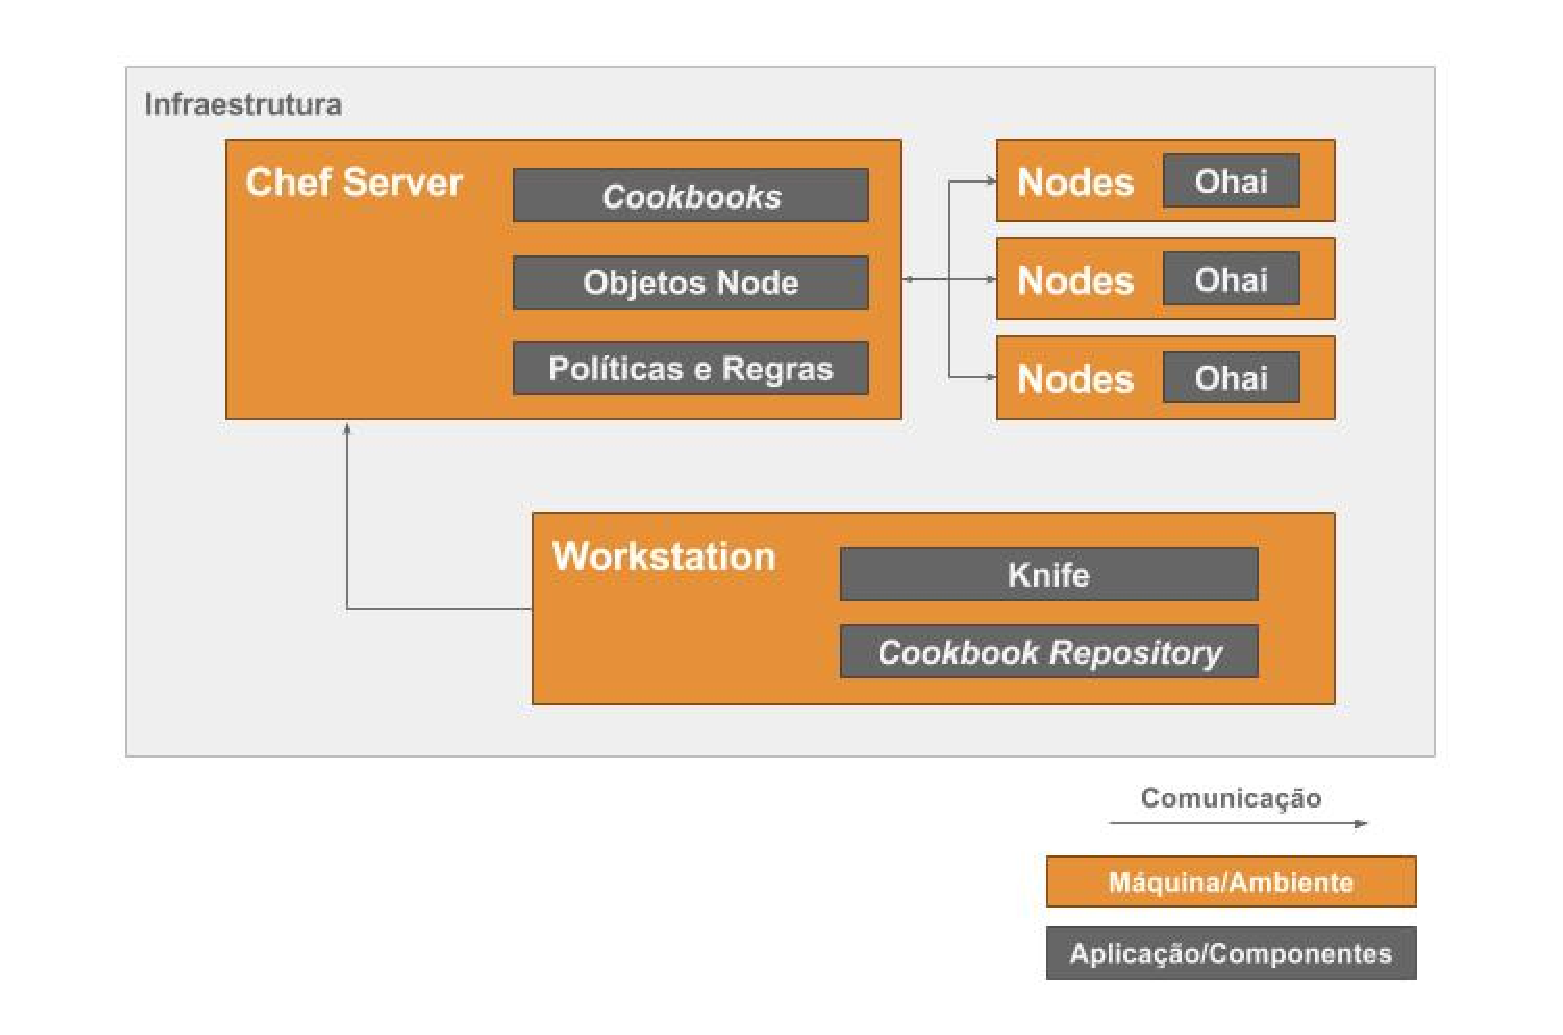
\includegraphics[width=0.9\textwidth]{figuras/chef-comp.eps}
\end{figure}

Chef utiliza os \textit{cookbooks} sendo a unidade básica de configuração do
ambiente. Neles são definidos comandos, arquivos, e outros atributos
para estabelecer o estado desejado para a instalação e configuração
do ambiente alvo \cite{sharma:2015}.

\citeonline{sharma:2015} Classifica os \textit{cookbooks} em três categorias:
\begin{itemize}
  \item \textbf{Aplicação}: contém as configurações de acordo com a instalação de
    uma aplicação. Exemplo PostgreSQL, Apache, Nginx;
  \item \textbf{Biblioteca}: define recursos a serem utilizados por outros \textit{cookbooks}
    (mais detalhes sobre recursos na seção~\ref{sec:lev-rec} no capítulo~\ref{chap:desenv} de desenvolvimento).
    Não é recomendado utilizado diretamente em um node;
  \item \textbf{\textit{Wrapper}}: são \textit{cookbooks} prontos construidos pela comunidade que podem
    ser alterados para que se adequem ao ambiente que será implantado.
\end{itemize}

O componente \textit{chef-client} irá executar as receitas (mais detalhes sobre receitas ou
\textit{recipes} na seção \ref{sec:lev-rec}) disponíveis nos \textit{cookbooks}
indicados pelo \textit{Chef Server} quando necessário, ou seja, se não houver
nenhuma mudança quanto as configurações do ambiente o \textit{chef-client} não irá
alterar nada, do contrário ele irá aplicar as configurações necessárias~\cite{chefdoc:2016}.




